\subsection{Kommunikation von Dateien innerhalb der Serveranwendung}
Alle Attribute, Parameter und Rückgaben, die im Entwurfsheft mit dem Typ "File" gekennzeichnet waren, haben wir jetzt als "Path" implementiert. Wobei wir die Klasse "Path" aus dem Modul "pathlib" der Python-Standardbibliothek importieren.

Im Folgenden soll die Handhabung der Dateien unter Zuhilfenahme von Pfaden erklärt werden. Dateien, die durch die API die oberste Schicht der Serverandwendung erreichen werden zunächst in einem temporären Ordner zwischen gespeichert. Der entsprechende Pfad im temporären Ordner wird entweder durch Aufruf eines Konstruktors in einem Objekt abgelegt oder unmittelbar an die Schnittstelle des Workflow-Packages übergeben.
Dort wird der Datei dann dem Aufruf entsprechend ein langfristiger Speicherort im Dateisystem zugewiesen. Die Löschung der Dateien im temporären Ordner obliegt dem Empfänger. Muss umgekehrt eine Datei vom Workflow-Package an die Schnittstelle der Serveranwendung gealngen, so wird der Pfad des langfristigen Speicherorts verwendet. Dort kann die Datei ausgelesen werden, gelöscht wird sie anschließend natürlich nicht.

Im Entwurfsheft haben wir uns keine Gedanken über die Ordnerstruktur der auf dem Server gespeicherten Dateien gemacht, deshalb reichen wir nun einen entsprechenden Entwurf nach. 

\begin{figure}[h]
            \label{Ordnerstruktur}
            \centerline{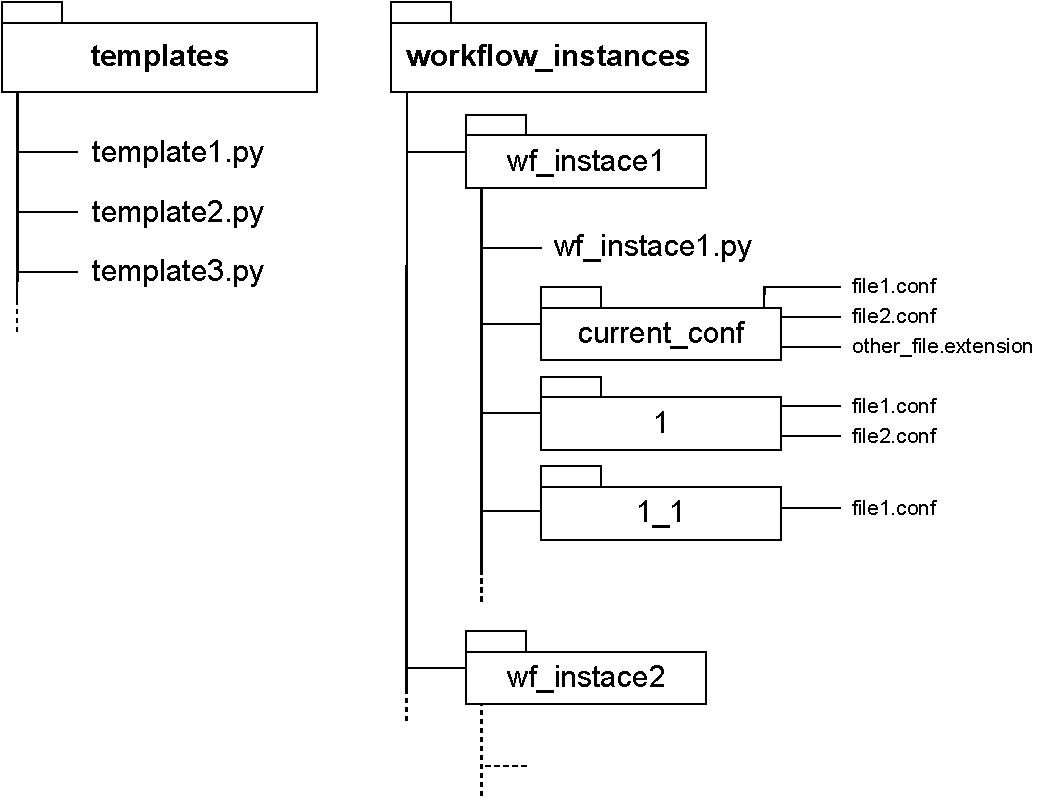
\includegraphics[scale=0.7]{res/ordnerstruktur.pdf}}
            \caption{Eine graphische Veranschaulichung der Ordnerstruktur}
        \end{figure}

Zum einen gibt es den Ordner "templates", der unmittelbar alle Dag-definition-files der bisher erstellten Templates enthält. Der Name der Datei stimmt dabei stets mit dem Namen des Templates überein. 

Daneben gibt es zudem noch den Ordner "workflow_instances". Dieser enthält für jede erstellte Workflow-Instanz einen Unterordner, der den eindeutigen Namen der Instanz trägt. In jedem dieser Unterordner befinden sich mindestens die Dag-definition-file der Instanz und der Ordner "current_conf", der in seiner Struktur stehts dem ursprünglich Konfigurationsordner enspricht. Insbesondere können auch Dateien mit einer Endung darin liegen, die nicht ".conf" ist. Die ".conf"-Dateien sind dabei immer auf dem Stand der aktuellen Version der Workflowinstanz. Ebenfalls fester Bestandteil ist der Ordner "1", der die initiale Version der Instanz representiert. In ihm liegen alle ".conf"-Dateien in ihrer ursprünglichen Fassung. Zusätzlich gibt es noch für jede neu erstellte Version einen Ordner, in dem stets nur die in dieser Version geänderten ".conf"-Dateien liegen.

\subsection{Änderungen im Workflow-Package}